\documentclass[]{article}
\usepackage{graphicx}
\usepackage{amsmath}

%opening
\title{N drones 1 package}
\author{Kien Huynh}

\begin{document}

\maketitle

\begin{abstract}

We consider the problem of package delivery using multiple drones in which each of their speeds can be different. There is one package and one destination, we need to find a good path and combination of drones so that the delivery time is as small as possible.

\end{abstract}

\section{Introduction}

Let $d_0$ to $d_{n-1}$ depict $n$ drones. Their starting positions are $p_0$ to $p_{n-1}$ and their speeds are $v_0$ to $v_{n-1}$. Without the loss of generality, assume that $v_0 < v_1 < ... < v_{n-1}$. The package is located at point $q_0$ and the location for delivery is $q_n$. Additionally, assume that $v_0$ can reach $q_0$ before any other drone (1). Two drones can exchange the package at some locations $q_i$. The problem here is to find the ordered set of optimal drones, their paths and their exchange locations so that the delivery time is the smallest. A note here is that in the optimal ordered set of drones will be monotonically increasing in speed as there is no point in handing the package to a slower drone (unless we are taking other factors such as battery or maximum traveling distance into account).

\section{Analysis for two drones}

\begin{figure}[!h]
	\centering
	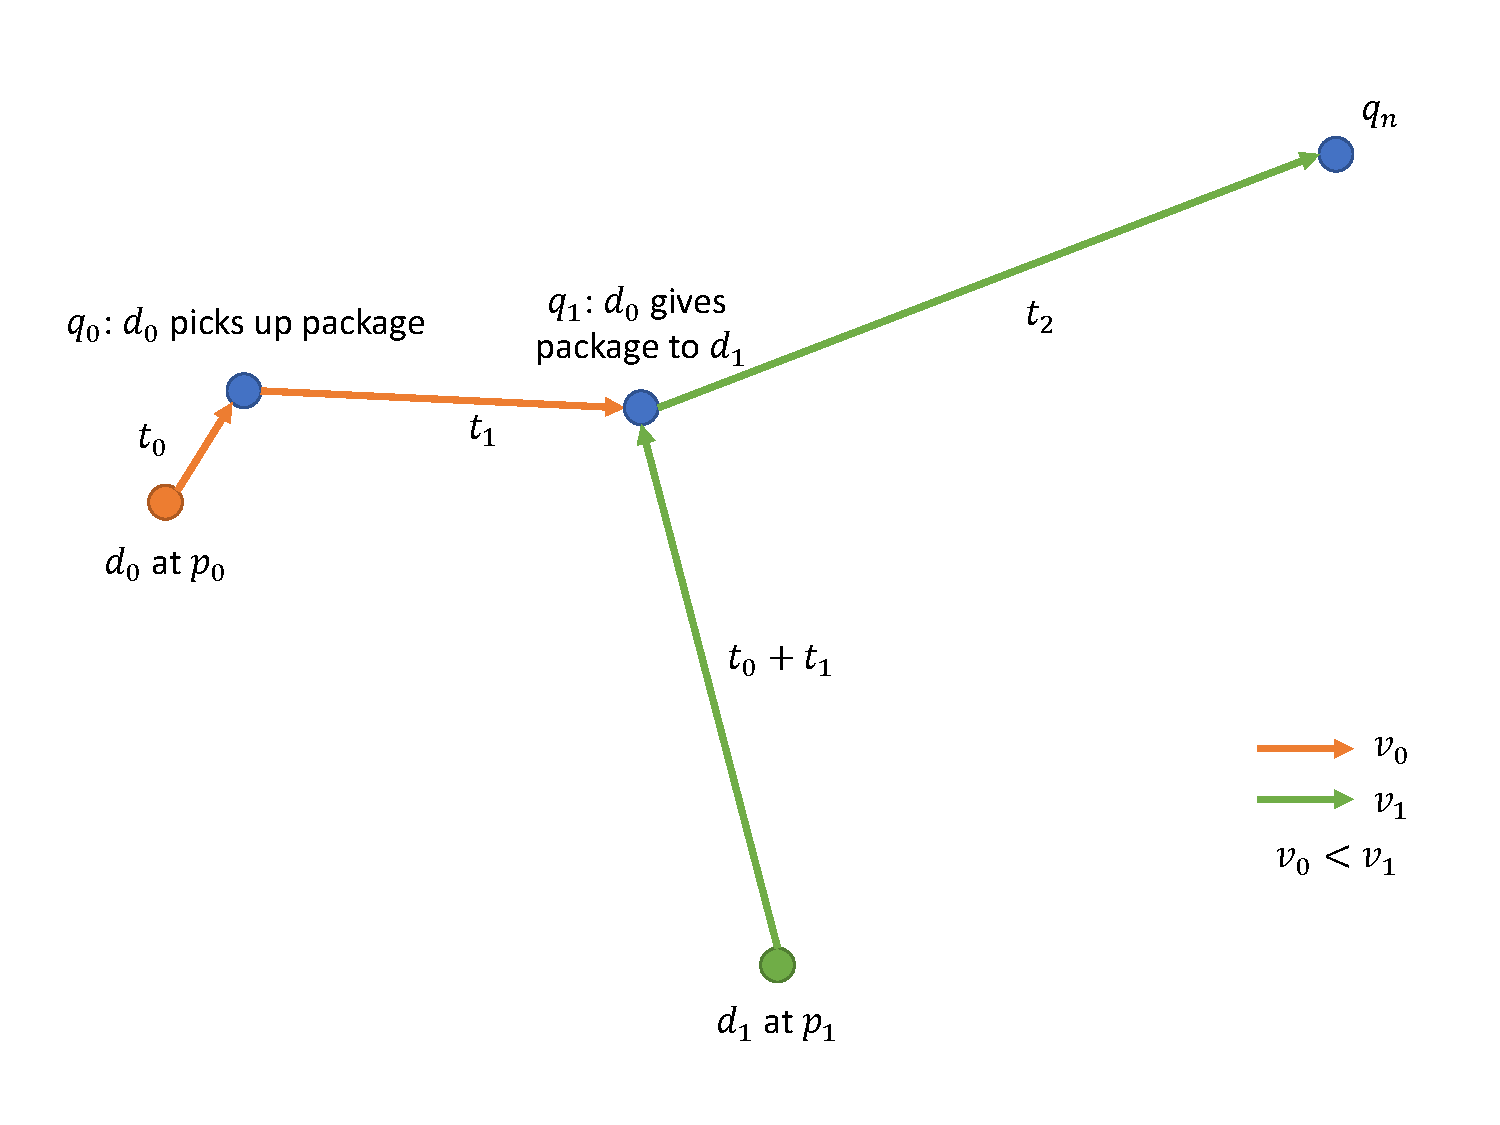
\includegraphics[width=10cm]{figures/2drones.pdf}
	\caption{Illustration of the case where there are only two drones.}
	\label{fig:2drone}
\end{figure}

Let:
\begin{itemize}
	\item $t_0$ be the time for $d_0$ to reach $q_0$ to get the package from the warehouse.
	\item $q_1$ be the location where $d_0$ and $d_1$ meet.
	\item $t_1$ be the time for $d_0$ to fly from $q_0$ to $q_1$. It's also the time for $d_1$ to fly from $p_1$ to $q_1$.
	\item $t_2$ be the time for $d_1$ to fly from $q_1$ to $q_n$ to deliver the package.
\end{itemize}

The details above are shown in Fig. \ref{fig:2drone}.

The goal is to minimize $t_0+t_1+t_2$ or $t_1+t_2$ because $t_0$ is a constant under assumption (1). The objective, written in term of speed and locations of the drones, is as follow:

\begin{align*}
\min_{q_1}\; &\frac{||q_1-p_1||}{v_1} + \frac{||q_1-q_n||}{v_1} \\
\textnormal{s.t.}\; &\frac{||q_1-q_0||}{v_0} + t_0 = \frac{||q_1-p_1||}{v_1}
\end{align*}

\begin{figure}[!h]
	\centering
	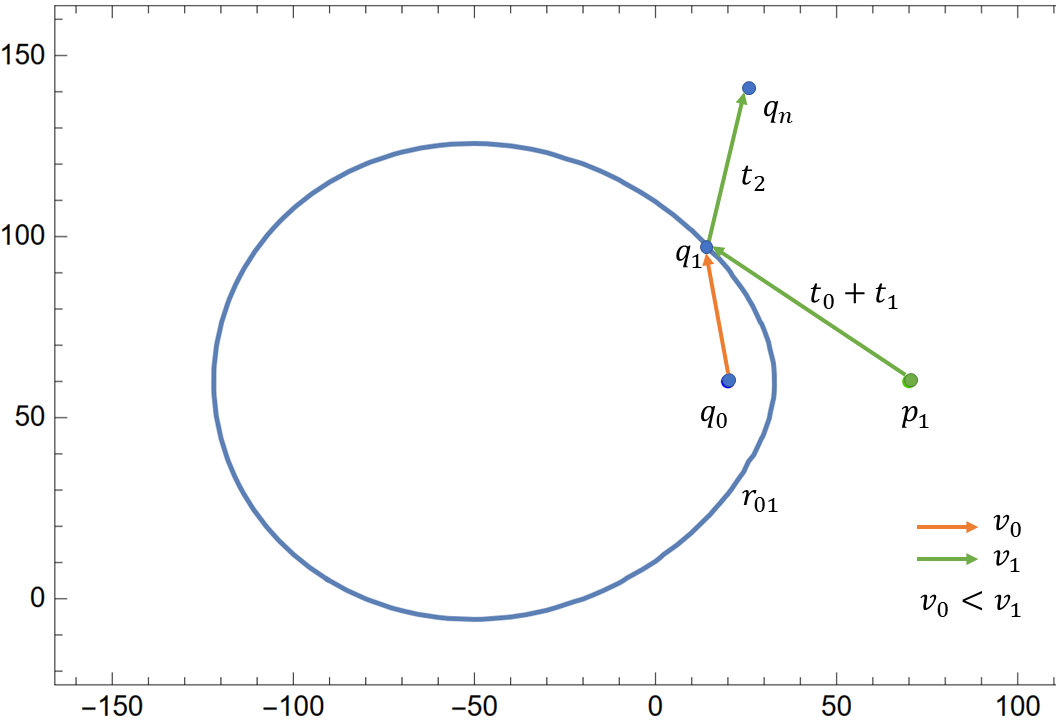
\includegraphics[width=10cm]{figures/2drones_q1qn.png}
	\caption{An example constraint: $\frac{1}{10}  \sqrt{{(x - 20)}^2 + {(y - 60)}^2} + 1.8 = \frac{1}{12} \sqrt{{(x - 70)}^2 + {(y - 60)}^2}, q_0=(20,60)$, $p1 = (70,60)$. $r_{01}$ is the set of all possible points where $d_0$ and $d_1$ could meet based on their speed.}
	\label{fig:2drone_q1}
\end{figure}

The constraint is there to ensure that the time it takes for $d_0$ and $d_1$ to go from their starting points to $q_1$ is the same. Let $r_{01}$ be the set of all possible $q_1$. The set $r_{01}$ is shown as a ring in Fig. \ref{fig:2drone_q1}. Another assumption here is that $q_n$ lies outside of $r_{01}$, otherwise there is no point in using $d_1$.

Geometrically, the objective is to find a point $q_1$ on the ring $r_{01}$ so that the distance $||q_1-p_1|| + ||q_n-q_1||$ is the smallest.

\section{Analysis for three drones}

In case there are three drones $d_0$, $d_1$ and $d_2$, one thing we can do at the start is checking if $r_{02}$ is completely contained by $r_{01}$. If it is, then we don't have to use $d_1$ since $d_2$ can meet $d_0$ faster. Otherwise, we can always use $d_1$ before $d_2$ (even if the ordered set $(d_0, d_2)$ gives the best result, inserting $d_1$ in-between can also give us the same best result). The reasoning is as follow:



\section{Analysis for the general case}



\end{document}
